\newpage
\genHeader

% This section applies to both??
\section{Creating Instances}

\hypertarget{creatingInstance common}{}Before diving into modelling dynamic behaviour in \texttt{Part III}, let's have a brief look at how to create a concrete \emph{instance model} of your metamodel in Eclipse.

In the following, we use \emph{metamodel} and \emph{instance model} to differentiate between models that represent the abstract syntax and static semantics of a domain specific language (metamodel), and those that are expressed \emph{in} such a language (instance models of the metamodel).

\begin{itemize}

\item[$\blacktriangleright$] To create an instance model, navigate to the generated \texttt{model} folder in your \texttt{LearningBoxLanguage} project. Double-click the \texttt{LearningBoxLanguage.ecore} model to invoke  the \emph{Ecore model editor}. The Eclipse Modeling Framework (EMF) provides a generic model editor for free that allows us to create and edit an arbitrary instance of any metamodel specified with eMoflon. Expand this tree to view the different classes and packages you modelled. 

\item[$\blacktriangleright$] To create a concrete instance of the metamodel, you must select a class which will become the root element of the new instance.
For our example, right-click the class \texttt{Box} and choose \texttt{Create Dynamic Instance\ldots} from the context-menu as depicted in figure.~\ref{fig:context_menu}.

\begin{figure}[htbp]
	\centering
  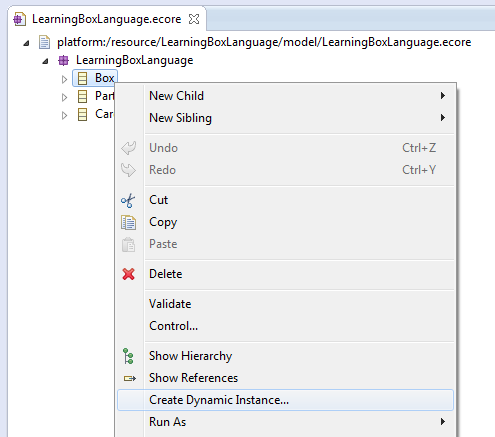
\includegraphics[width=0.6\textwidth]{eclipse_createInstance}
	\caption{Context menu of Ecore model in Eclipse}
	\label{fig:context_menu}
\end{figure}


\item[$\blacktriangleright$] A dialogue should appear asking where the instance model file should be persisted. We suggest saving all your instances in a folder named \texttt{instances} that is created in every new repository project. This is however just a convention, you are of course free to store your instances anywhere. Last but not least, enter a name for the instance model (Fig.~\ref{fig:store_dynamic_instance}).

\begin{figure}[htbp]
	\centering
  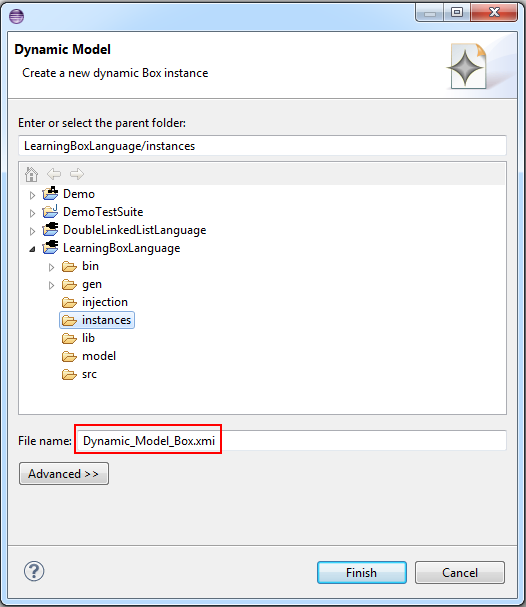
\includegraphics[width=0.5\textwidth]{eclipse_boxDynamicModel}
	\caption{Dialogue for creating a dynamic model instance}
	\label{fig:store_dynamic_instance}
\end{figure}

\item[$\blacktriangleright$] Press \texttt{Finish} and the \emph{generic model editor} should be opened for your instance model.
This editor works just like the previous Ecore model editor, but it is ``generic,'' meaning it allows you to create and edit an instance of \emph{any} metamodel, not just of Ecore.

\item[$\blacktriangleright$] You can populate your instance model by adding new children or siblings via a right-click on an element of the instance model to invoke the context-menu depicted in figure~\ref{fig:create_instance}.
Note that EMF supports you by respecting your metamodel and reducing the choice of creatable elements to valid types only\footnote{This depends on the current context. Try it out!}.

\begin{figure}[htbp]
	\centering
  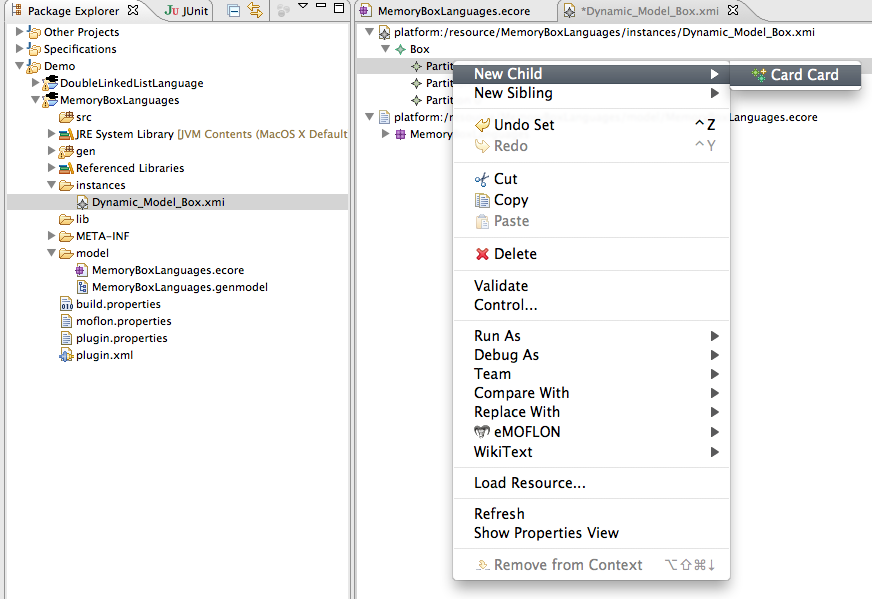
\includegraphics[width=0.9\textwidth]{adjustModel}
	\caption{Context menu for creating model elements}
	\label{fig:create_instance}
\end{figure}

\item[$\blacktriangleright$] You can save your model as an XMI file by pressing \texttt{Ctrl+S}.
The model can be reloaded via a simple double-click to invoke the generic model editor.

\item[$\blacktriangleright$] Lets try building a vocabulary set. Fill your box with two partitions, with three cards in each. Your ecore tree should now resemble figure~\ref{fig:eclipse_populatedTree}.

\begin{figure}[htbp]
	\centering
  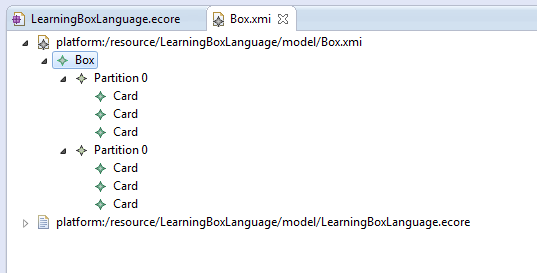
\includegraphics[width=0.6\textwidth]{eclipse_populatedTree}
	\caption{Our Learning Box with two filled partitions.}
	\label{fig:eclipse_populatedTree}
\end{figure}

\vfill
\pagebreak

\item[$\blacktriangleright$] Double click on one of the partitions to bring up the ``Properties'' tab in the window below the editor. Here you'll see the attributes you defined earlier in the classes! Pick a number - any one you like - and edit the `Index' value. As soon as you hit `Enter,' you'll see that the change in name has been reflected in the tree. Give the seond partition a unique EInt value.

\item[$\blacktriangleright$] In the same fashion, double click on each \texttt{Card} you created and modify their values. In particular, modify the 'Back' attribute - this is the name you'll see from the partition.

\item[$\blacktriangleright$] You now have a unique, customized learning box! Ensure no errors exist before proceeding with the final part of this tutorial.

\end{itemize}

\fancyfoot[R]{ $\triangleright$ \hyperlink{conclusion}{Next} }